%%% Una plantilla para elaborar trabajo y tareas
%%% Luis O. Ramírez Fernández < lramirez88mx@comunidad.unam.mx>
%%% La vesión más reciente en https://github.com/opengraphix/plantilla_tareas_LATEX
%%%
%%% ------------------------------------------------------------------------
%%% Requerimientos:
%%% ------------------------------------------------------------------------
%%% cite
%%% apacite
%%% spanish
%%% latin1
%%% enumerate
%%% graphicx
%%% float
%%% array
%%% amsmath
%%% amssymb
%%% helvet
%%%
%%% ------------------------------------------------------------------------
%%% Opcioal
%%% ------------------------------------------------------------------------
%%% git
%%% vc.sty
%%%
%%% ------------------------------------------------------------------------
%%% Notas
%%%------------------------------------------------------------------------
%%%
%%%
%%%------------------------------------------------------------------------

\documentclass[letterpaper, 12pt, spanish]{article}

%% Citas en formato APA
\usepackage{cite} %Referenciar citas en biblitex
\usepackage{apacite}

%% Esto es para poder escribir acentos directamente:
\usepackage[utf8]{inputenc}
\usepackage{enumerate}

%% Esto es para que LaTeX sepa que el texto está en español:
\usepackage[spanish,activeacute]{babel}

%% Para imágenes, tablas y flotantes
\usepackage{graphicx, float, array}

%% Para matemáticas
\usepackage{amsmath, amssymb}

%% Parametros para margenes del documento
%\usepackage[right=2.5cm,left=2.5cm,top=2.5cm,bottom=2.5cm,headsep=0cm,footskip=1cm]{geometry}
\usepackage[width=150mm,top=25mm,bottom=25mm,bindingoffset=6mm]{geometry}
%\setlength{\parskip}{\baselineskip} %Espaciado entre cada párrafo
\renewcommand{\baselinestretch}{1.5} %Espaciado de línea 1.5 puntos
\usepackage[T1]{fontenc}

%%%------------------------------------------------------------------------
%%% Tipografia:
%%%------------------------------------------------------------------------
%% Se pueden utilizar la siguientes fuentes Helvetica, Charter, Avante Grade,
%% Palatino y Verdana
%% Solo descomenta o comenta la que te agrade, segun sea el caso


%% Charter
%\usepackage{charter} %% Charter
%\renewcommand{\familydefault}{bch}
%% Palatino
\usepackage{palatino} %% Palatino
\renewcommand{\familydefault}{ppl}
%% Avant Grade
%\usepackage{avant} %% Avant Grade
%\renewcommand{\familydefault}{pag}
%% Helvetica
%\usepackage{helvet} %% Helvetica
%\renewcommand{\familydefault}{phv}

%%%------------------------------------------------------------------------
%%% Metadatos
%%%------------------------------------------------------------------------

%% Modifica a tus necesidades.
\author{Nombre Paterno Materno}
\title{Título de la tarea}
%\date{}

%%%------------------------------------------------------------------------
%%% Registro de versiones con Git
%%%------------------------------------------------------------------------

%% Si no quieres usar git o el paquete vc (desde CTAN), comenta la linea correspondientes.
%% Si comentas, debes estar seguro de comentar toda la secci�n
%\immediate\write18{sh ./vc}
%%%% This file has been generated by the vc bundle for TeX.
%%% Do not edit this file!
%%%
%%% Define Git specific macros.
\gdef\GITHash{269215527be6f137e29ca079d3564336f923d906}%
\gdef\GITAbrHash{2692155}%
\gdef\GITParentHashes{}%
\gdef\GITAbrParentHashes{}%
\gdef\GITAuthorName{Luis Octavio Ramírez Fernández}%
\gdef\GITAuthorEmail{opengraphix@opengraphix.com.mx}%
\gdef\GITAuthorDate{2016-03-02 19:27:48 -0600}%
\gdef\GITCommitterName{Luis Octavio Ramírez Fernández}%
\gdef\GITCommitterEmail{opengraphix@opengraphix.com.mx}%
\gdef\GITCommitterDate{2016-03-02 19:27:48 -0600}%
%%% Define generic version control macros.
\gdef\VCRevision{\GITAbrHash}%
\gdef\VCAuthor{\GITAuthorName}%
\gdef\VCDateRAW{2016-03-02}%
\gdef\VCDateISO{2016-03-02}%
\gdef\VCDateTEX{2016/03/02}%
\gdef\VCTime{19:27:48 -0600}%
\gdef\VCModifiedText{\textcolor{red}{with local modifications!}}%
%%% Assume clean working copy.
\gdef\VCModified{0}%
\gdef\VCRevisionMod{\VCRevision}%

%\usepackage{scrpage2}
%  \pagestyle{scrheadings}
%  \lefoot{rev: \VCRevision}
%  \lofoot{rev: \VCRevision}
%  \refoot{fecha mod: \VCDateTEX}
%  \rofoot{fecha mod: \VCDateTEX }

%%%------------------------------------------------------------------------
%%% Cuerpo del Documento
%%%------------------------------------------------------------------------

\begin{document}
\maketitle

\section{Introducción}
Lorem ipsum dolor sit amet, consectetur adipiscing elit. Praesent vehicula porta diam et volutpat. Nam mattis facilisis pulvinar. Donec consectetur pulvinar ullamcorper. Aenean ac eleifend dolor. Sed imperdiet enim id ligula tempor, eget hendrerit ex commodo. Etiam dapibus fermentum rutrum. Sed sit amet pulvinar dui. Class aptent taciti sociosqu ad litora torquent per conubia nostra, per inceptos himenaeos. In volutpat sem lacus, sit amet scelerisque dui consectetur quis. Nullam luctus elit ac laoreet vulputate. Mauris metus nisl, ultricies in diam eget, faucibus accumsan arcu. Quisque eget blandit nibh, in facilisis quam.

Proin eleifend ex id neque pharetra, sit amet interdum massa lobortis. Phasellus sit amet ullamcorper nisl. Nulla lobortis est vel consectetur molestie. Nunc ac feugiat lacus. Ut velit mi, faucibus in lacinia bibendum, facilisis ac ex. Aliquam congue feugiat fringilla. Nulla nisi metus, dignissim sed ex nec, luctus lacinia sapien. Praesent auctor dapibus ipsum sit amet vulputate. Vestibulum semper tempus laoreet. Donec tempus ligula at nisl ultricies, eget efficitur enim elementum. Nullam aliquet ultrices rutrum. In a massa in nunc auctor interdum eu vel ante. Etiam quam enim, rutrum ut ornare non, efficitur ut ligula. Ut non pellentesque augue.

In sit amet metus sapien. Donec a massa consequat purus accumsan finibus quis a dui. Aenean mauris elit, bibendum nec est vitae, consequat ultrices ligula. Suspendisse ac accumsan est. Aliquam faucibus nisl vitae lacinia pretium. Proin non vulputate nunc. Nullam quis lacinia lectus, nec bibendum enim. Duis quam magna, rutrum sit amet elit nec, scelerisque finibus nunc.

Fusce ultricies tincidunt risus, nec rutrum lacus accumsan non. Quisque suscipit velit in nibh finibus commodo. Proin fringilla at lacus et venenatis. Quisque congue accumsan nisl, eu malesuada tellus placerat at. Donec euismod, dui quis viverra ornare, metus velit imperdiet turpis, quis pharetra lectus felis ut dui. Etiam ultricies tincidunt neque id finibus. Nulla a mi et dolor suscipit finibus. Vestibulum dui nulla, sagittis non nisl euismod, blandit rutrum eros. Praesent eget lectus est. Ut vitae luctus dolor.


\section{Desarrollo del tema}

Lorem ipsum dolor sit amet, consectetur adipiscing elit. Praesent vehicula porta diam et volutpat. Nam mattis facilisis pulvinar. Donec consectetur pulvinar ullamcorper. Aenean ac eleifend dolor. Sed imperdiet enim id ligula tempor, eget hendrerit ex commodo. Etiam dapibus fermentum rutrum. Sed sit amet pulvinar dui. Class aptent taciti sociosqu ad litora torquent per conubia nostra, per inceptos himenaeos. In volutpat sem lacus, sit amet scelerisque dui consectetur quis. Nullam luctus elit ac laoreet vulputate. Mauris metus nisl, ultricies in diam eget, faucibus accumsan arcu. Quisque eget blandit nibh, in facilisis quamn  \cite{kaplan1999}.

Proin eleifend ex id neque pharetra, sit amet interdum massa lobortis. Phasellus sit amet ullamcorper nisl. Nulla lobortis est vel consectetur molestie. Nunc ac feugiat lacus. Ut velit mi, faucibus in lacinia bibendum, facilisis ac ex. Aliquam congue feugiat fringilla. Nulla nisi metus, dignissim sed ex nec, luctus lacinia sapien. Praesent auctor dapibus ipsum sit amet vulputate. Vestibulum semper tempus laoreet. Donec tempus ligula at nisl ultricies, eget efficitur enim elementum. Nullam aliquet ultrices rutrum. In a massa in nunc auctor interdum eu vel ante. Etiam quam enim, rutrum ut ornare non, efficitur ut ligula. Ut non pellentesque augue.

\subsection{Subsección del tema}
Lorem ipsum dolor sit amet, consectetur adipiscing elit. Praesent vehicula porta diam et volutpat. Nam mattis facilisis pulvinar. Donec consectetur pulvinar ullamcorper. Aenean ac eleifend dolor. Sed imperdiet enim id ligula tempor, eget hendrerit ex commodo. Etiam dapibus fermentum rutrum. Sed sit amet pulvinar dui. Class aptent taciti sociosqu ad litora torquent per conubia nostra, per inceptos himenaeos. In volutpat sem lacus, sit amet scelerisque dui consectetur quis. Nullam luctus elit ac laoreet vulputate. Mauris metus nisl, ultricies in diam eget, faucibus accumsan arcu \cite{marr2015}. Quisque eget blandit nibh, in facilisis quam.

Proin eleifend ex id neque pharetra, sit amet interdum massa lobortis. Phasellus sit amet ullamcorper nisl. Nulla lobortis est vel consectetur molestie. Nunc ac feugiat lacus. Ut velit mi, faucibus in lacinia bibendum, facilisis ac ex. Aliquam congue feugiat fringilla. Nulla nisi metus, dignissim sed ex nec, luctus lacinia sapien. Praesent auctor dapibus ipsum sit amet vulputate. Vestibulum semper tempus laoreet. Donec tempus ligula at nisl ultricies, eget efficitur enim elementum. Nullam aliquet ultrices rutrum. In a massa in nunc auctor interdum eu vel ante. Etiam quam enim, rutrum ut ornare non, efficitur ut ligula. Ut non pellentesque augue.

In sit amet metus sapien. Donec a massa consequat purus accumsan finibus quis a dui. Aenean mauris elit, bibendum nec est vitae, consequat ultrices ligula. Suspendisse ac accumsan est. Aliquam faucibus nisl vitae lacinia pretium. Proin non vulputate nunc. Nullam quis lacinia lectus, nec bibendum enim. Duis quam magna, rutrum sit amet elit nec, scelerisque finibus nunc.

\section{Otro tema o sección}
Colocar viñetas:
\begin{enumerate} % Inicia enumeraci�n
 \item \textbf{Punto 1}, In sit amet metus sapien. Donec a massa consequat purus accumsan finibus quis a dui. Aenean mauris elit, bibendum nec est vitae, consequat ultrices ligula.
 \item \textbf{Punto 2}, cIn sit amet metus sapien. Donec a massa consequat purus accumsan finibus quis a dui. Aenean mauris elit, bibendum nec est vitae, consequat ultrices ligula.
 \item \textbf{Punto 3},In sit amet metus sapien. Donec a massa consequat purus accumsan finibus quis a dui. Aenean mauris elit, bibendum nec est vitae, consequat ultrices ligula.
 \item \textbf{Punto 4}, In sit amet metus sapien. Donec a massa consequat purus accumsan finibus quis a dui. Aenean mauris elit, bibendum nec est vitae, consequat ultrices ligula \cite{marr2015}.
\end{enumerate}

%Colocar una imagen
\begin{figure}[H]
\begin{center}
  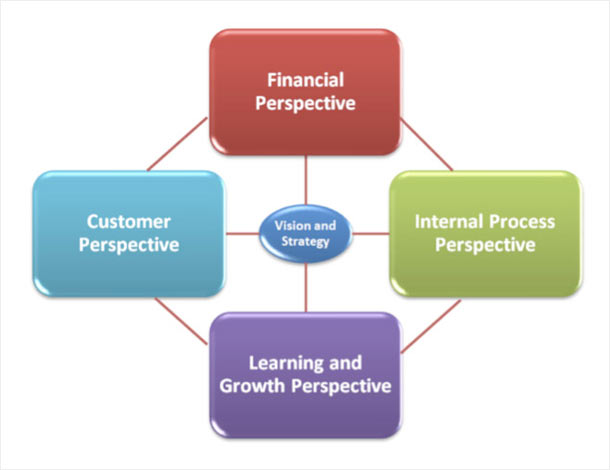
\includegraphics[width=200px]{./images/bsc1.jpg}
  \caption{Perspectivas del Cuadro de Mando Integrador}
\end{center}
\end{figure}

\subsection{Subsección del tema}
Lorem ipsum dolor sit amet, consectetur adipiscing elit. Praesent vehicula porta diam et volutpat. Nam mattis facilisis pulvinar. Donec consectetur pulvinar ullamcorper. Aenean ac eleifend dolor. Sed imperdiet enim id ligula tempor, eget hendrerit ex commodo. Etiam dapibus fermentum rutrum. Sed sit amet pulvinar dui. Class aptent taciti sociosqu ad litora torquent per conubia nostra, per inceptos himenaeos. In volutpat sem lacus, sit amet scelerisque dui consectetur quis. Nullam luctus elit ac laoreet vulputate. Mauris metus nisl, ultricies in diam eget, faucibus accumsan arcu. Quisque eget blandit nibh, in facilisis quam \cite{baraybar2011}.


\section{Conclusiones}
Lorem ipsum dolor sit amet, consectetur adipiscing elit. Praesent vehicula porta diam et volutpat. Nam mattis facilisis pulvinar. Donec consectetur pulvinar ullamcorper. Aenean ac eleifend dolor. Sed imperdiet enim id ligula tempor, eget hendrerit ex commodo. Etiam dapibus fermentum rutrum. Sed sit amet pulvinar dui. Class aptent taciti sociosqu ad litora torquent per conubia nostra, per inceptos himenaeos. In volutpat sem lacus, sit amet scelerisque dui consectetur quis. Nullam luctus elit ac laoreet vulputate. Mauris metus nisl, ultricies in diam eget, faucibus accumsan arcu. Quisque eget blandit nibh, in facilisis quam.


% Bibliografía.
%-----------------------------------------------------------------
% para agregar más referencias es necesario abrir el archivo : biblio/bibliografia.bib
% Compilar las referencias desde la línea de comandos o terminal:
% $ latex PaternoMatenoN_plantillatarea
% $ bibtex PaternoMatenoN_plantillatarea
% $ latex PaternoMatenoN_plantillatarea
% $ latex PaternoMatenoN_plantillatarea
%-----------------------------------------------------------------

\bibliography{biblio/bibliografia.bib}
\setlength{\parindent}{-0.2in}
\setlength{\leftskip}{0.2in}
\setlength{\parskip}{8pt}
\vspace*{-0.2in}
\noindent
\bibliographystyle{apacite}


\end{document}
